\documentclass{beamer}  
\usepackage{amsmath}
\usepackage{graphicx}
\usepackage{url}
\usepackage{color}

\makeatletter
\def\url@smallurlstyle{%
 \@ifundefined{selectfont}{\def\UrlFont{\sf}}{\def\UrlFont{\footnotesize\ttfamily}}}
\makeatother
\urlstyle{smallurl}

\mode<presentation>
{ \usetheme{Darmstadt} }

\title{Mesh Networking for in Cave Communications}

\institute{Open SDR}
\author{Philip Balister\inst{1} \and
Paul Walko\inst{2}}
\institute{\inst{1} OpenSDR {\tt\tiny philip@opensdr.com} \and \inst{2} Big Cave Maps {\tt\tiny paul@bigcavemaps.com}}

\date{June 26, 2024}
 
\begin{document} 

\begin{frame}
\titlepage
\end{frame}

\section*{Outline}

\begin{frame}
  \tableofcontents
\end{frame}

\section{Background}

\begin{frame}
\frametitle{Current state of the art in cave communciations}

\begin{itemize}
\item United States: Military field phones
\item Europe: Through the earth communications
	\begin{itemize}
	\item Low frequency (below 500 kHz)
	\item Heyphone: voice only
	\item Cavelink: text only
	\item Both are not available at the moment
	\end{itemize}
\item \tiny\url{https://caverescue.eu/documents/communication/communications-catalogue/}
\item \tiny\url{https://radiolocation.weebly.com/}
\end{itemize}

\end{frame}

\begin{frame}
\frametitle{Operational Challenges}

\begin{itemize}
	\item Existing wired and wireless systems are point to point
	\item Military field phones are purchased from the surplus market
	\item Wireless solutions have large antennas
	\item Prototype solutions exist, but ruggedized packaging is challenging
\end{itemize}

\end{frame}

\begin{frame}
\frametitle{Underground Wireless Networks}

\begin{itemize}
	\item APRS Cave-link, demonstrated in 2013
	\item Sybet SpellCom system
	\item BuecherNet, designed for sensor data
	\item \tiny\url{http://aprs.org/cave-link.html}
	\item \tiny\url{https://sybet.eu/spellcom/}
	\item \tiny\url{https://caves.org/webinars/buechernet-fortstanton-nm/}
\end{itemize}
\end{frame}

\section{Meshtastic}

\begin{frame}
\frametitle{Meshtastic}

\begin{center}
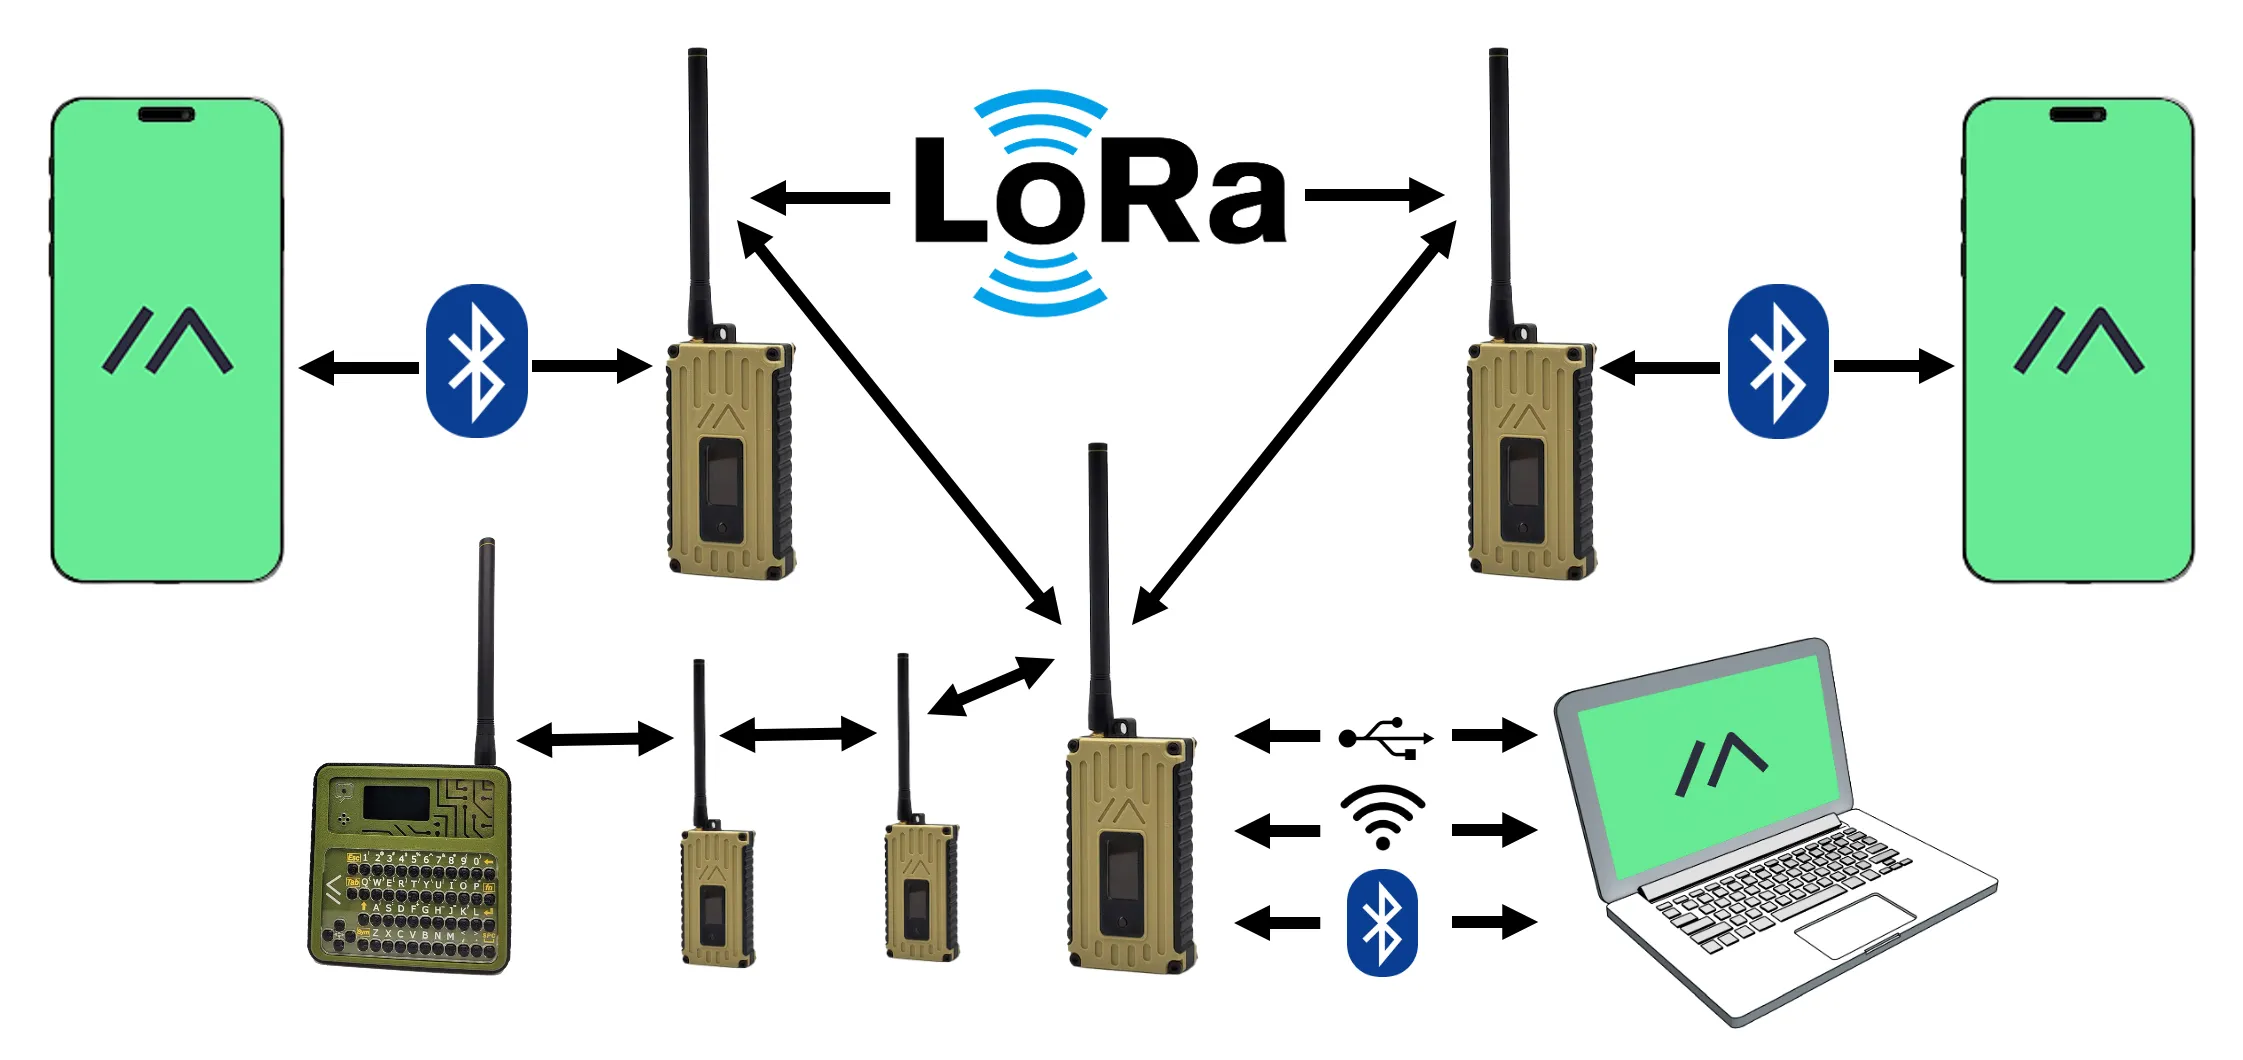
\includegraphics[width=4.0in]{../images/lora-topology-2.png}
\end{center}

\end{frame}


\begin{frame}
	\frametitle{Field Test Results}

\begin{center}
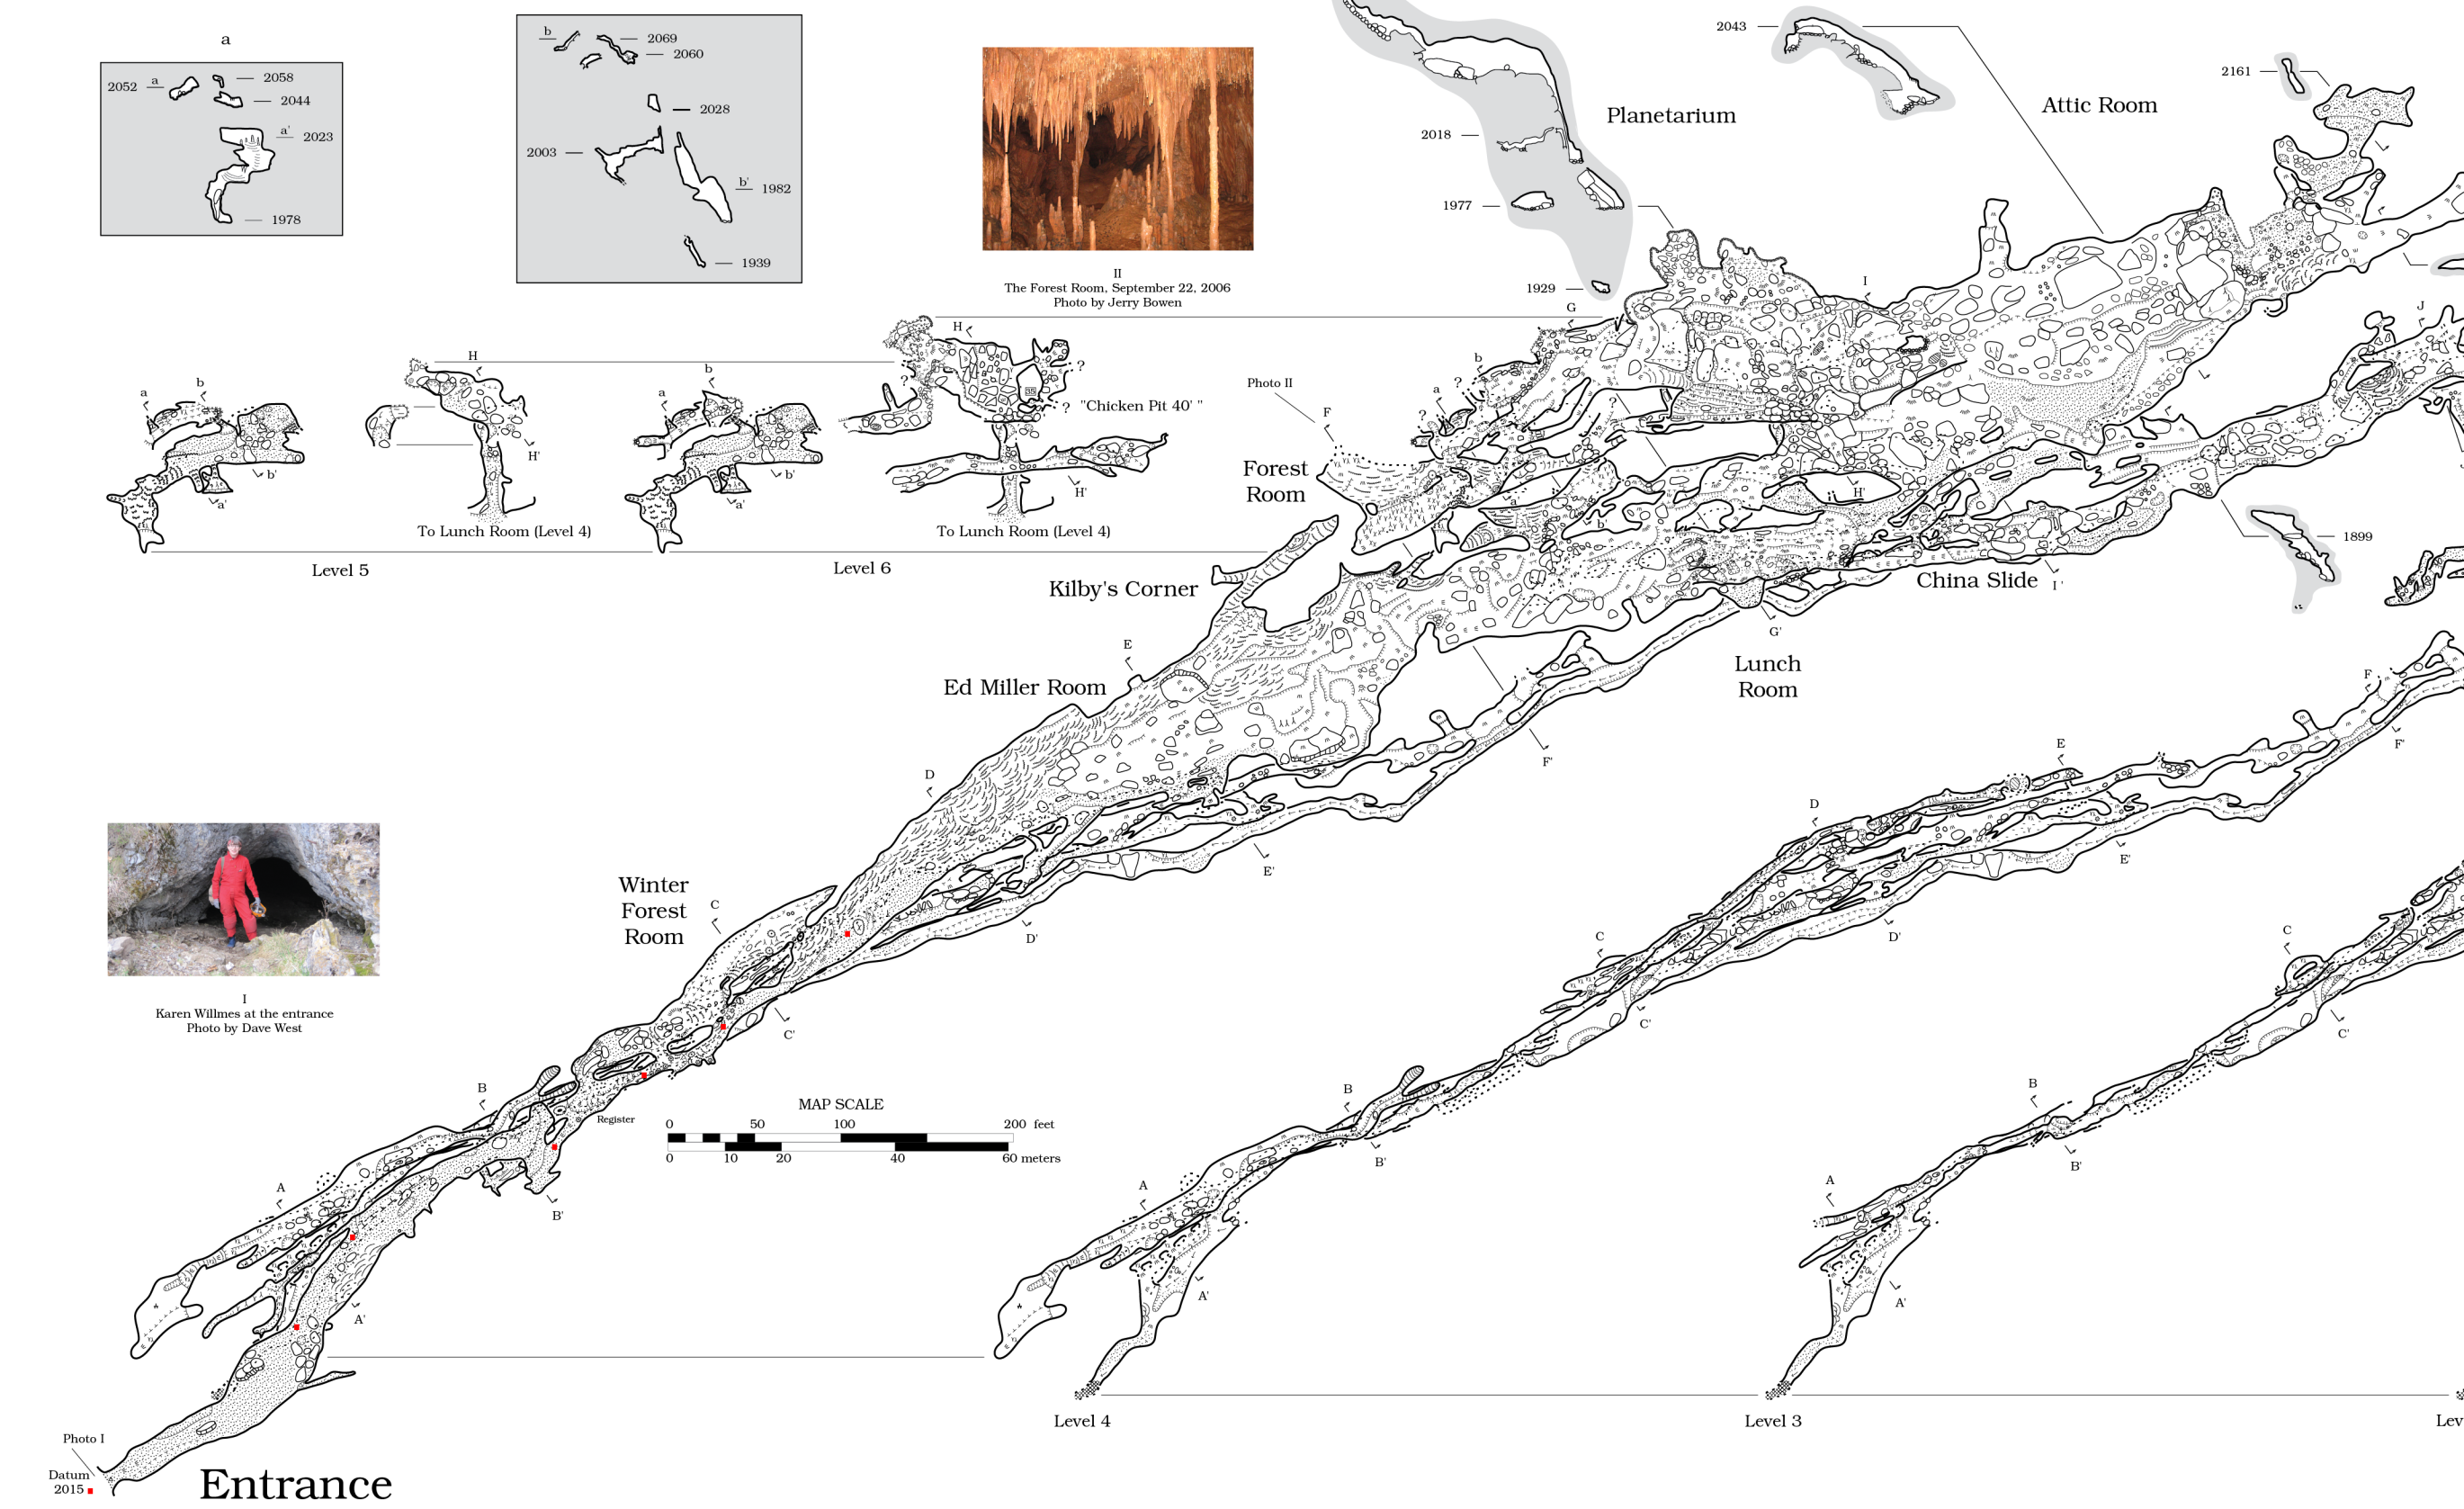
\includegraphics[width=4.0in]{../images/New-River-June-4-2024.png}
\end{center}

\end{frame}


\begin{frame}
	\frametitle{Excitement!}

%\begin{center}
%\includegraphics[width=3.0in]{../images/Excitement.png}
%\end{center}

\end{frame}
\begin{frame}

	\frametitle{OpenEmbedded and the Yocto Project}

\begin{itemize}
\item In 2010, the Yocto Project is announced at ELCE in Cambridge, UK
\begin{itemize}
	\item The first of many Linux Foundation Collaborative Projects
\end{itemize}
\item The Yocto Project provides an organization for corporate entities to join
\item OpenEmbedded is the Yocto Project technical partner
\item OpenEmbedded has a representative on Yocto Project governing board.
\item Both organizations have Technical Steering committees
\item OpenEmbedded represents the people in the community
\item Confusing? Yes it is.
\end{itemize}

\end{frame}


\begin{frame}
	\frametitle{Current OpenEmbedded Leadership (1)}

	\begin{itemize}
		\item Four member board, three year terms
			\begin{itemize}
				\item Philip Balister (Crofton) (Oct 2020)
				\item Denys Dmytriyenko (denix) (Oct 2021)
				\item Jon Mason (jonmason) (Oct 2022)
				\item Jan-Simon Moeller (dl9pf) (Oct 2022)
			\end{itemize}
	\end{itemize}
\end{frame}


\begin{frame}
	\frametitle{Current OpenEmbedded Leadership (2)}

	\begin{itemize}
		\item Five member technical steering committee, two year terms
			\begin{itemize}
				\item Bruce Ashfield (zeddii) (Sep 2023)
				\item Jon Mason (jonmason) (Sep 2023)
				\item Joshua Watt (JPEW) (Sep 2023)
				\item Paul Eggleton (bluelightning) (Sep 2023)
				\item Richard Purdie (RP) (Sep 2023)
			\end{itemize}
	\end{itemize}
\end{frame}


\begin{frame}
\frametitle{What really changed}

\begin{itemize}
	\item OpenEmbedded Classic had one layer for all recipe.
		\begin{itemize}
			\item Yes I know about collections
		\end{itemize}
	\item Many developers had push access
	\item Uneven testing
	\item No concept of a release
	\item Everyone was frustrated
\end{itemize}

\end{frame}

\begin{frame}
\frametitle{Process Improvements}

\begin{itemize}
	\item OpenEmbedded-core created with a subset of recipes
	\item Layer concept extendeded to collect recipes into subsets
	\item OpenEmbedded-core tests patches before the merge
	\item Yocto Project dues fund autobuilder for large testing matrix
	\item Two releases per year
\end{itemize}

\end{frame}


\section{Present}

\begin{frame}
\frametitle{The Good}

\begin{itemize}
\item Core layers build consistently
\item Healthy job market for developers
\item Layers are available for broad spectrum of software
\item You can do anything you want
\end{itemize}

\end{frame}

\begin{frame}
\frametitle{The Bad}

\begin{itemize}
\item You can do anything you want
\item Error reporting can be confusing
\item Usability issues persist
\end{itemize}

\end{frame}

\section{Future}

\begin{frame}
\frametitle{The next ten years!}

\begin{itemize}
\item What features do we need?
\item How do we get new people involved?
\item How do we communicate with end users?
\end{itemize}

\end{frame}


\begin{frame}
	\frametitle{Become an OpenEmbedded Member}

	\begin{itemize}
		\item Membership open to all with an interest in OpenEmbedded
		\item Benefits of membership ...
		\item Responsibilities of membership.
			\begin{itemize}
				\item Vote for OpenEmbedded board members
				\item Vote for OpenEmbedded Technical Steering Committee members
				\item Vote for Yocto Project Technical Steering Committee members
			\end{itemize}
		\item Becoming a member.
			\begin{itemize}
				\item Send a paragraph about who you are and your involvement
				\item To board@openembedded.org
				\item The members then approve the new members
			\end{itemize}
	\end{itemize}
\end{frame}


\begin{frame}
	\frametitle{Encourage your company to join the Yocto Project}

	\begin{itemize}
		\item Dues support several areas.
			\begin{itemize}
				\item Developers
				\item Infrastructure
				\item Advocacy
				\item Community
				\item Training/Developer days
				\item Administration/Legal
			\end{itemize}
		\item Recognition for your company.
		\item Contact Nicolas Dechesne $<$nicolas.dechesne@linaro.org$>$
	\end{itemize}
\end{frame}


\begin{frame}
\frametitle{Questions}

Answer my Questions!

\end{frame}

\end{document}
